

\title{A numerical tour of wave propagation: Finite difference implemenation}
\renewcommand{\thefootnote}{\fnsymbol{footnote}}
\author{Pengliang Yang\footnotemark[1]\\
\footnotemark[1]Xi'an Jiaotong University, Xi'an, China, 710049
}
\usetikzlibrary{decorations.pathreplacing} 
\usetikzlibrary{scopes}

\righthead{Primer for wave propagation}
\lefthead{Pengliang Yang}

\maketitle
\begin{abstract}
 This tutorial is written for beginners as an introduction to basic wave propagation using finite difference method, from acoustic and elastic wave modeling, to reverse time migration and full waveform inversion. Most of the theoretical delineations summarized in this tutorial have been implemented in Madagascar with Matlab, C and CUDA programming, which will benefit readers' further study.
\end{abstract}

\section{Basic wave equation}

Define  $\textbf{x}=(x,y,z)$, time $t$, the $s$-th energy source function $ \tilde{S}(\textbf{x},t;\textbf{x}_s) $, pressure $p(\textbf{x},t; \textbf{x}_s)$, particle velocity $ \textbf{v}(\textbf{x},t) $, material density $ \rho(\textbf{x}) $, the bulk modulus $\kappa(\textbf{x})$. Now we have
\begin{description}
	\item $\bullet$ Newton's law
	\begin{equation}\label{eq:newton}
	\rho(\textbf{x})\frac{\partial\textbf{v}(\textbf{x},t;\textbf{x}_s)}{\partial t}=\nabla p(\textbf{x},t;\textbf{x}_s).
	\end{equation}

	\item $\bullet$ Constitutive law
	\begin{equation}\label{eq:constitutive}
	\frac{1}{\kappa(\textbf{x})}\frac{\partial p(\textbf{x},t;\textbf{x}_s)}{\partial t}=\nabla \cdot \textbf{v}(\textbf{x},t;\textbf{x}_s)+\tilde{S}(\textbf{x},t;\textbf{x}_s).
	\end{equation}
\end{description}

\subsection{Acoustic wave equation}

Acoustics is a special case of fluid dynamics (sound waves in gases and liquids) and linear elastodynamics. Note that elastodynamics is a more accurate representation of earth dynamics, but most industrial seismic processing based on acoustic model. Recent interest in quasiacoustic anisotropic approximations to elastic P-waves.

Assume $\tilde{S}(\textbf{x},t;\textbf{x}_s)$ is differentiable constitutive law w.r.t. time $t$.
Substituting Eq. \eqref{eq:constitutive} into the differentiation of Eq. \eqref{eq:newton}  gives
\begin{equation}
\frac{1}{\kappa(\textbf{x})}\frac{\partial^2 p(\textbf{x},t;\textbf{x}_s)}{\partial t^2}
=\nabla\cdot \left(\frac{1}{\rho(\textbf{x})}\nabla p(\textbf{x},t; \textbf{x}_s)\right)
+\frac{\partial \tilde{S}(\textbf{x},t;\textbf{x}_s)}{\partial t}.
\end{equation}
We introduce $ v(\textbf{x})=\sqrt{\kappa(\textbf{x})/\rho(\textbf{x})} $ (compressional p-wave velocity):
\begin{equation}
\frac{1}{v^2(\textbf{x})}\frac{\partial^2 p(\textbf{x},t;\textbf{x}_s)}{\partial t^2}
=\rho(\textbf{x}) \nabla\cdot \left(\frac{1}{\rho(\textbf{x})}\nabla p(\textbf{x},t; \textbf{x}_s)\right)
+\rho(\textbf{x})\frac{\partial\tilde{S}(\textbf{x},t;\textbf{x}_s)}{\partial t}
\end{equation}
Under constant density condition, we obtain the 2nd-order equation
\begin{equation}\label{eq:scalar_wav}
\frac{1}{v^2(\textbf{x})}\frac{\partial^2 p(\textbf{x},t;\textbf{x}_s)}{\partial t^2}=\nabla^2 p(\textbf{x},t;\textbf{x}_s)+f_s(\textbf{x},t;\textbf{x}_s)
\end{equation}
where $\nabla^2=\nabla\cdot\nabla=\frac{\partial^2}{\partial x^2}+\frac{\partial^2}{\partial z^2}$, $f_s(\textbf{x},t;\textbf{x}_s)=\rho(\textbf{x})\frac{\partial\tilde{S}(\textbf{x},t;\textbf{x}_s)}{\partial t}$. In 2D case, it is
\begin{equation}
 \frac{\partial^2 p(\textbf{x},t;\textbf{x}_s)}{\partial t^2}
 =v^2(\textbf{x})\left(\frac{\partial^2 p(\textbf{x},t;\textbf{x}_s) }{\partial z^2} 
 +\frac{\partial^2 p(\textbf{x},t;\textbf{x}_s)}{\partial x^2}\right)+f_s(\textbf{x},t;\textbf{x}_s).
\end{equation}
A shot of acoustic wavefield obtained at t=0.35s with 4-th order finite difference scheme and the sponge absorbing boundary condition is shown in Figure~\ref{fig:snapfd2d}, where the source is put at the center of the model. For 3D, it becomes
\begin{equation}
 \frac{\partial^2 p(\textbf{x},t;\textbf{x}_s)}{\partial t^2}
 =v^2(\textbf{x})\left(\frac{\partial^2 p(\textbf{x},t;\textbf{x}_s) }{\partial z^2}  
 +\frac{\partial^2 p(\textbf{x},t;\textbf{x}_s)}{\partial x^2}
 +\frac{\partial^2 p(\textbf{x},t;\textbf{x}_s)}{\partial y^2}\right)+f_s(\textbf{x},t;\textbf{x}_s)
\end{equation}
Similarly, we put the source at the center of a 3D volume (size=100x100x100), performed the modeling for 300 steps in time and recorded the corresponding wavefield at kt=250, see Figure~\ref{fig:snapfd3d}.

% 
% \begin{figure}
%   \centering
%   % Requires \usepackage{graphicx}
%   \includegraphics[width=0.6\textwidth]{snapfd2d}\\
%   \caption{A snap of acoustic wavefield obtained at t=0.35s with 4-th order finite difference scheme and the sponge absorbing boundary condition.}\label{fig:snapfd2d}
% \end{figure}
% 
% 
% \begin{figure}
%   \centering
%   % Requires \usepackage{graphicx}
%   \includegraphics[width=0.6\textwidth]{snapfd3d}\\
%   \caption{A wavefield snap recorded at kt=250, 300 steps modeled.}\label{fig:snapfd3d}
% \end{figure}



\inputdir{testfd2d}
\plot{snapfd2d}{width=0.6\textwidth}{A snap of acoustic wavefield obtained at t=0.35s with 4-th order finite difference scheme and the sponge absorbing boundary condition.}

\inputdir{testfd3d}
\plot{snapfd3d}{width=0.6\textwidth}{A wavefield snap recorded at kt=250, 300 steps modeled.}

The above spatial operator is spatially homogeneous. This isotropic formula is simple and  easy to understand, and becomes the basis for many complicated generalizations in which the anisotropy may come in. In 2D case, the elliptically-anisotropic wave equation reads
\begin{equation}
 \frac{\partial^2 p(\textbf{x},t;\textbf{x}_s)}{\partial t^2}
 =v_1^2(\textbf{x})\frac{\partial^2 p(\textbf{x},t;\textbf{x}_s) }{\partial z^2} 
 +v_2^2(\textbf{x})\frac{\partial^2 p(\textbf{x},t;\textbf{x}_s)}{\partial x^2}+f_s(\textbf{x},t;\textbf{x}_s)
\end{equation}
Here, I use the Hess VTI model shown in Figure~\ref{fig:vp} and Figure~\ref{fig:vx}. We perform 1000 steps of modeling with time interval $\Delta t=0.001s$, and capture the wavefield at $t=0.9s$, as shown in Figure~\ref{fig:snapaniso}. 

% 
% \begin{figure}
%   \centering
%   \includegraphics[width=0.75\textwidth]{vp}
%   \caption{Hess VTI model: velocity component 1.}\label{fig:vp}
% \end{figure}
% 
% \begin{figure}
%   \centering
%   \includegraphics[width=0.75\textwidth]{vx}
%   \caption{Hess VTI model: velocity component 2.}\label{fig:vx}
% \end{figure}
% 
% \begin{figure}
%   \centering
%   \includegraphics[width=0.75\textwidth]{snapaniso}\\
%   \caption{Wavefield at $kt=0.9s$, 1000 steps of modeling with time interval $\Delta t=0.001s$ performed.}
%   \label{fig:snapaniso}
% \end{figure}

\inputdir{testaniso}
\multiplot{2}{vp,vx}{width=0.45\textwidth}{Two velocity components of Hess VTI model}
\plot{snapaniso}{width=0.5\textwidth}{Wavefield at $kt=0.9s$, 1000 steps of modeling with time interval $\Delta t=0.001s$ performed.}



\subsection{Elastic wave equation}

In elastic wave equation, the modulus $\kappa(\textbf{x})$ corresponds to two Lame parameters: $\lambda+2\mu=\rho v_p^2$ and $u=\rho v_s^2$, in which $v_p$ and $v_s$ denote the P- and S-wave velocity. The elastic wave equation can be written as
\begin{equation}\label{eq:elastic}
\left\{
\begin{split}
	\frac{\partial v_x}{\partial t} &=\frac{1}{\rho} (\frac{\partial \tau_{xx}}{\partial x}+\frac{\partial \tau_{xz}}{\partial x})\\
	\frac{\partial v_z}{\partial t} &=\frac{1}{\rho} (\frac{\partial \tau_{zx}}{\partial z}+\frac{\partial \tau_{zz}}{\partial z})\\	
	\frac{\partial\tau_{xx}}{\partial t} &=(\lambda+2\mu)\frac{\partial v_x}{\partial x}+\lambda\frac{\partial v_z}{\partial z}\\
	\frac{\partial\tau_{zz}}{\partial t} &=\lambda\frac{\partial v_x}{\partial x}+(\lambda+2\mu)\frac{\partial v_z}{\partial z}\\
	\frac{\partial\tau_{xz}}{\partial t} &=\mu \frac{\partial v_x}{\partial x}+\mu\frac{\partial v_z}{\partial z}\\
\end{split}\right.
\end{equation}
where $\tau_{ij}$ (sometimes $\sigma_{ij}$) is stress, $v_i$ is particle velocity, $i,j=x,z$. We display the 2 components of elastic wave propagation at $kt=270$, $nt=300$ modeled with $\Delta t=0.001$ in Figure~\ref{fig:elasticxz}, in which the grid size is 200x200, the spatial interval is $\Delta x=\Delta z=5m$, and the velocities are chosen to be $Vp=2km/s$, $Vs=Vp/\sqrt{2}$.

% 
% \begin{figure*}
%   \centering
%   \includegraphics[width=\textwidth]{elasticxz}\\
%   \caption{Two components of elastic wave propagation at $kt=270$, $nt=300$ modeled with $\Delta t=0.001$. Grid size=200x200,$\Delta x=\Delta z=5m$, $Vp=2km/s$, $Vs=Vp/\sqrt{2}$}
%   \label{fig:elasticxz}
% \end{figure*}


\inputdir{testelastic2d}
\plot{elasticxz}{width=\textwidth}{Two components of elastic wave propagation at $kt=270$, $nt=300$ modeled with $\Delta t=0.001$. Grid size=200x200,$\Delta x=\Delta z=5m$, $Vp=2km/s$, $Vs=Vp/\sqrt{2}$}

\section{Forward modeling}

\subsection{Taylor and P\'{a}de expansion}

The Taylor expansion of a function $f(x+h)$ at $x$ is written as
\begin{equation}
f(x+h)=f(x)+\frac{\partial f(x)}{\partial x}h+\frac{1}{2!}\frac{\partial^2 f(x)}{\partial x^2}h^2+\frac{1}{3!}\frac{\partial^3 f(x)}{\partial x^3}h^3+\ldots.
\end{equation}
A popular example is
\begin{equation}
(1+x)^{\alpha}=1+\alpha x+\frac{\alpha(\alpha-1)}{2!}x^2+\ldots+\frac{\alpha(\alpha-1)\cdots(\alpha-n+1)}{n!}x^n+\ldots.
\end{equation}
Here we mainly consider the following expansion formula:
\begin{equation}\label{eq: taylor1}
(1-x)^{\frac{1}{2}}=1-\frac{1}{2}x-\frac{1}{8}x^2-\frac{1}{16}x^3-\frac{5}{128}x^4-\ldots, |x|<1.
\end{equation}

The P\'{a}de expansion of Eq. \eqref{eq: taylor1} follows from expansion in continuous fractions:
\begin{equation}
(1-x)^{\frac{1}{2}}=1-\frac{x/2}{1-\frac{x/4}{1-\frac{x/4}{\ldots}}}
\end{equation}
I provide an informal derivation:
\begin{displaymath}
\begin{split}
y&=(1-x)^{\frac{1}{2}}\Rightarrow x=1-y^2=(1-y)(1+y)\Rightarrow 1-y=\frac{x}{1+y}\\
y&=1-\frac{x}{1+y}=1-\frac{x}{1+(1-\frac{x}{1+y})}=1-\frac{x/2}{1-\frac{x/2}{1+y}}\\
&=1-\frac{x/2}{1-\frac{x/2}{2-\frac{x}{1+y}}}
=1-\frac{x/2}{1-\frac{x/4}{1-\frac{x/2}{1+y}}}=\ldots
\end{split}
\end{displaymath}
The 1st-order Pade expansion is:
\begin{equation}
(1-x)^{\frac{1}{2}}=1-\frac{x}{2}
\end{equation}
The 2nd-order Pade expansion is:
\begin{equation}
(1-x)^{\frac{1}{2}}=1-\frac{x/2}{1-\frac{x}{4}}.
\end{equation}
And the 3rd-order one is:
\begin{equation}
(1-x)^{\frac{1}{2}}=1-\frac{x/2}{1-\frac{x/4}{1-\frac{x}{4}}}.
\end{equation}

\subsection{Approximate the wave equation}

The innovative work was done by John Claerbout, and is well-known as $15^{\circ}$ wave equation to separate the up-going and down-going waves \citep{claerbout1971toward,claerbout1986imaging}.

Eliminating the source term, the Fourier transform of the scalar wave equation (Eq. \eqref{eq:scalar_wav}) can be specified as:
\begin{equation}
\frac{\omega^2}{v^2}=k_x^2+k_z^2.
\end{equation}
The down-going wave equation in Fourier domain is
\begin{equation}
k_z=\sqrt{\frac{\omega^2}{v^2}-k_x^2}=\frac{\omega}{v}\sqrt{1-\frac{v^2k_x^2}{\omega^2}}.
\end{equation}
Using the different order Pade expansions, we have:
\begin{equation}\left\{
\begin{split}
\mathrm{1st-order:} &k_z=\frac{\omega}{v}\left(1-\frac{v^2k_x^2}{2\omega^2}\right)\\
\mathrm{2nd-order:} &k_z=\frac{\omega}{v}\left(1-\frac{\frac{2v^2k_x^2}{\omega^2}}{4-\frac{v^2k_x^2}{\omega^2}}\right)\\
\mathrm{3rd-order:} &k_z=\frac{\omega}{v}\left(1-\frac{\frac{v^2k_x^2}{2\omega^2}-\frac{v^4 k_x^4}{8\omega^4}}{1-\frac{v^2k_x^2}{2\omega^2}}\right)\\
\mathrm{4th-order:} &k_z=\frac{\omega}{v}\left(1-\frac{\frac{v^2k_x^2}{2\omega^2}-\frac{v^4 k_x^4}{4\omega^4}}{1-\frac{3v^2k_x^2}{4\omega^2}+\frac{v^4k_x^4}{16\omega^4}}\right)\\
\end{split}\right.
\end{equation}
The corresponding time domain equations are:
\begin{equation}\left\{
\begin{split}
&\mathrm{1st-order:}
\frac{\partial^2 p}{\partial z^2}+\frac{v}{2}\frac{\partial^2 p}{\partial x^2}
-\frac{1}{v}\frac{\partial^2 p}{\partial t^2}=0, \mathrm{(the \, well-known\, 15^{\circ}\, wave\, equation)}\\
&\mathrm{2nd-order:}
\frac{\partial^3 p}{\partial t^2\partial z}-\frac{v^2}{4}\frac{\partial^3 p}{\partial x^2\partial z}-\frac{1}{v}\frac{\partial^3 p}{\partial t^3}+\frac{3v}{4}\frac{\partial^3 p}{\partial x^2\partial t}=0,  \mathrm{(45^{\circ}\, wave\, equation)}\\
&\mathrm{3rd-order:}
\frac{\partial^4 p}{\partial t^3\partial z}-\frac{v^2}{2}\frac{\partial^4 p}{\partial x^2\partial t\partial z}-\frac{1}{v}\frac{\partial^4 p}{\partial t^4}+v\frac{\partial^4 p}{\partial x^2\partial t^2}-\frac{v^3}{8}\frac{\partial^4 p}{\partial x^4}=0\\
&\mathrm{4th-order:}
\frac{\partial^5 p}{\partial t^4\partial z}-\frac{3v^2}{4}\frac{\partial^5 p}{\partial x^2\partial t^2\partial z}-\frac{v^4}{16}\frac{\partial^5 p}{\partial x^4\partial z}
+\frac{1}{v}\frac{\partial^5 p}{\partial t^5}
+\frac{5v}{4}\frac{\partial^5 p}{\partial x^2\partial t^3}+\frac{5v^3}{16}\frac{\partial^5 p}{\partial t\partial x^4}=0\\
\end{split}\right.
\end{equation}

\subsection{Absorbing boundary condition (ABC)}

\subsubsection{Clayton-Enquist boundary condition}

To simulate the wave propagation in the infinite space, the absorbing boundary condition (ABC), namely the proximal approximation (PA) boundary condition,  was proposed in \cite{clayton1977absorbing} and \cite{engquist1977absorbing}. The basic idea is to use the wave equation with opposite direction at the boundary. Take the bottom boundary as an example. Here, allowing for the incident wave is down-going, we use the up-going wave equation at the bottom boundary. Using a model including 3 layers (Figure~\ref{fig:vel}), Figure~\ref{fig:shots} displays 10 shots data volume obtained the Clayton-Enquist boundary condition.

% 
% \begin{figure*}
%   \centering
%   \includegraphics[width=0.6\textwidth]{vel}\\
%   \caption{Velocity model: 3 layers}
%   \label{fig:vel}
% \end{figure*}
% 
% \begin{figure*}
%   \centering
%   \includegraphics[width=0.6\textwidth]{shots}\\
%   \caption{10 shots data volume obtained using the Clayton-Enquist boundary condition.}
%   \label{fig:shots}
% \end{figure*}

\inputdir{modeling2d}

\plot{vel}{width=0.6\textwidth}{Velocity model: 3 layers}
\plot{shots}{width=0.6\textwidth}{10 shots data volume obtained using the Clayton-Enquist boundary condition.}


\subsubsection{Sponge ABC}

The sponge ABC was proposed by \cite{cerjan1985nonreflecting}. The principle is very simple: attenuating the refections exponentially in the extended artificial boundary (Figure~\ref{fig:extbndr}) area by multiplying a factor less $d(u)$ than 1. Commonly, we use the factor
\begin{equation}
d(u)=\mathrm{exp}(-[0.015*(nb-i)]^2), u=x,z (i\Delta x \; \mathrm{or} \; i\Delta z)
\end{equation}
where $nb$ is the thickness of the artificial boundary on each side of the model. Usually, we choose it to be $nb=20 \sim30$.
The sponge ABC can be easily applied to a wide range of wave propagation problems, including some  governing wave equations for complicated medium. 

% \begin{figure}
%   \centering
%   % Requires \usepackage{graphicx}
%   \includegraphics[width=0.5\textwidth]{pml}\\
%   \caption{A schematic diagram of extended artificial boundary area}\label{fig:pml}
% \end{figure}

%\inputdir{../}
%\plot{pml}{width=0.6\textwidth}{A schematic diagram of extended artificial boundary area}


\begin{figure}
  \centering
  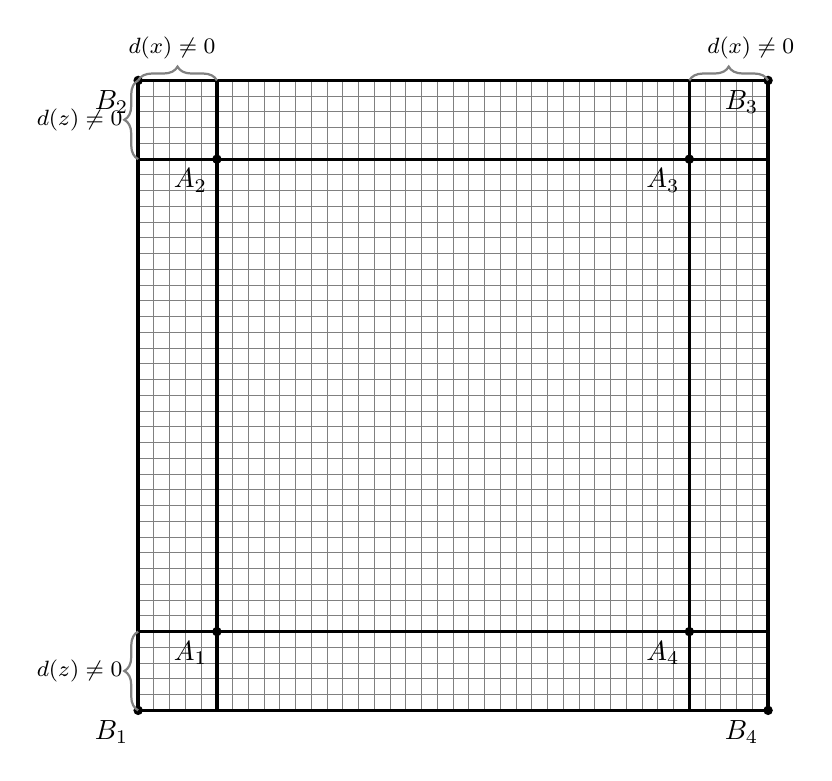
\begin{tikzpicture}
    \draw[step=0.2cm,color=gray] (-4,-4) grid (4,4);
    \draw[below left] (-3,-3) node(s){$A_1$};
    \draw[below left] (-3,3) node(s){$A_2$};
    \draw[below left] (3,3) node(s){$A_3$};
    \draw[below left] (3,-3) node(s){$A_4$};
    \draw[below left] (-4,-4) node(s){$B_1$};
    \draw[below left] (-4,4) node(s){$B_2$};
    \draw[below left] (4,4) node(s){$B_3$};
    \draw[below left] (4,-4) node(s){$B_4$};
    \draw[very thick] (-3,-4)--(-3,4);    
    \draw[very thick] (3,-4)--(3,4);
    \draw[very thick] (-4,3)--(4,3);    
    \draw[very thick] (-4,-3)--(4,-3);
    \draw[very thick] (-4,-4)--(-4,4)--(4,4)--(4,-4)--cycle;   
    \fill (-3,-3) circle (0.06cm) (-3,3) circle (0.06cm) (3,3) circle (0.06cm) (3,-3)circle (0.06cm);
    \fill (-4,-4) circle (0.06cm) (-4,4) circle (0.06cm) (4,4) circle (0.06cm) (4,-4)circle (0.06cm); 
    
    \draw [thick,gray,decorate,decoration={brace,amplitude=5pt}] (-4,4)  -- (-3,4) 
      node [black,midway,above=4pt,xshift=-2pt] {\footnotesize $d(x)\neq 0$};
    \draw [thick,gray,decorate,decoration={brace,amplitude=5pt}] (3,4) -- (4,4)
      node [black,midway,above=4pt,xshift=8pt] {\footnotesize $d(x)\neq 0$};
    \draw [thick,gray,decorate,decoration={brace,amplitude=5pt}] (-4,-4)  -- (-4,-3) 
      node [black,midway,left=10pt,xshift=8pt] {\footnotesize $d(z)\neq 0$};
    \draw [thick,gray,decorate,decoration={brace,amplitude=5pt}] (-4,3) -- (-4,4)
      node [black,midway,left=10pt,xshift=8pt] {\footnotesize $d(z)\neq 0$};
  \end{tikzpicture}
  \caption{A schematic diagram of extended artificial boundary area. $A_1A_2A_3A_4$ is the original model zone, which is extended to be $B_1B_2B_3B_4$  with artificial boundary. In the extended bounary area, the attenuation coeffcient $d(u)\neq 0$; In the model zone $A_1A_2A_3A_4$, $d(u)= 0$, $u=x,z$. }\label{fig:extbndr}
\end{figure}



\subsection{Perfectly Matched Layer (PML)}

The PML ABC was proposed in electromagnetics computation \citep{berenger1994perfectly}. In seismic wave propagration community, two  versions of PML boundary condition have been developed: the split PML (SPML) and nonsplit PML (NPML).

\subsubsection{Split PML (SPML) for acoustics}

It is possible for us to split the wave field into two components: x-component $p_x$ and z-component $p_z$ \citep{carcione2002seismic}. Then the acoustic wave equation becomes 
\begin{equation}\label{eq:spml}
\left\{
\begin{split}
	p=&p_x +p_z\\
	\frac{\partial p_x}{\partial t}=& v^2 \frac{\partial v_x}{\partial x}\\
	\frac{\partial p_z}{\partial t}=& v^2 \frac{\partial v_z}{\partial z}\\
	\frac{\partial v_x}{\partial t}=& \frac{\partial p}{\partial x}\\
	\frac{\partial v_z}{\partial t}=& \frac{\partial p}{\partial z}
\end{split}
\right.
\end{equation}
To absorb the boundary reflection, by adding the decaying coefficients $d(u)$ the SPML governing equation can be specified as \citep{collino2001application}
\begin{equation}\label{eq:spml}
\left\{
\begin{split}
	p=p_x +p_z&\\
	\frac{\partial p_x}{\partial t}+d(x)p_x &= v^2 \frac{\partial v_x}{\partial x}\\
	\frac{\partial p_z}{\partial t}+d(z)p_z &= v^2 \frac{\partial v_z}{\partial z}\\
	\frac{\partial v_x}{\partial t}+d(x)v_x &= \frac{\partial p}{\partial x}\\
	\frac{\partial v_z}{\partial t}+d(z)v_z &= \frac{\partial p}{\partial z}
\end{split}
\right.
\end{equation}
where $d(x)$ and $d(z)$ are the ABC coefficients designed to attenuate the reflection in the boundary zone, see Figure~\ref{fig:extbndr}. There exists many forms of ABC coefficients function. In the absorbing layers, we use the following
model for the damping parameter $d(x)$ \citep{collino2001application}:
\begin{equation}
 d(u)=d_0(\frac{u}{L})^2, d_0=-\frac{3v}{2L}\ln(R), u=x,z
\end{equation}
where $ L$ indicates the PML thinkness; $x$ represents the distance between current position (in PML) and PML inner boundary. $R$ is always chosen as $10^{-3}\sim 10^{-6}$. It is important to note that the same idea can be applied to elastic wave equation \citep{collino2001application}. The split version of wave equation is very suitable for the construction of seismic Poynting vector. A straightforward application is the angle gather extration using Poynting vector, see Section \ref{sec:imaging_condition}.

A numerical example of SPML using 8th order staggered finite difference scheme is given in Figure~\ref{fig:snapspml}.

% 
% \begin{figure*}
%   \centering
%   \includegraphics[width=0.6\textwidth]{snapspml}\\
%   \caption{Wavefield snap of SPML with 8th order finite difference }
%   \label{fig:snapspml}
% \end{figure*}
% 

\inputdir{testspml}
\plot{snapspml}{width=0.6\textwidth}{Wavefield snap of SPML with 8th order finite difference }


\subsubsection{Nonsplit Convolutional-PML (CPML) for acoustics}

Another approach to improve the behavior of the discrete PML at grazing incidence consists in modifying the complex coordinate transform used classically in the PML to introduce a frequency-dependent term that implements a Butterworth-type filter in the layer. This approach has been developed for Maxwell’s equations  named convolutional PML (CPML) \citep{roden2000convolutional} or complex frequency shifted-PML (CFS-PML). The key idea is that for waves whose incidence is close to normal, the presence of such a filter changes almost nothing because absorption is already almost perfect. But for waves with grazing incidence, which for geometrical reasons do not penetrate very deep in the PML, but travel there a longer way in the direction parallel to the layer, adding such a filter will strongly attenuate them and will prevent them from leaving the PML with significant energy .

Define $Ax=\frac{\partial p}{\partial x}$, $Az=\frac{\partial p}{\partial z}$. Then the acoustic wave equation reads
\begin{displaymath}
\frac{\partial^2 p}{\partial t^2}=v^2\left(\frac{\partial Ax}{\partial x}+\frac{\partial Az}{\partial z}\right).
\end{displaymath}
To combine the absorbing effects into the acoustic equation, we merely need to combine two convolution terms into the above equations:
\begin{equation}
\left\{
\begin{split}
\frac{\partial^2 p}{\partial t^2}&=v^2\left(Px+Pz\right)\\
Px&=\frac{\partial Ax}{\partial x}+\Psi_x\\
Pz&=\frac{\partial Az}{\partial z}+\Psi_z\\
Ax&=\frac{\partial p}{\partial x}+\Phi_x\\
Az&=\frac{\partial p}{\partial z}+\Phi_z
\end{split}
\right.
\end{equation}
where $\Psi_x$, $\Psi_z$ are the convolution terms of $Ax$ and $Az$; $\Phi_x$, $\Phi_z$ are the convolution terms of $Px$ and $Pz$. These convolution terms can be computed via the following relation:
\begin{equation}
\left\{
\begin{split}
\Psi_x^n=b_x \Psi_x^{n-1}+(b_x-1) \partial_x^{n-1/2}Ax\\
\Psi_z^n=b_z \Psi_z^{n-1}+(b_z-1) \partial_z^{n-1/2}Az\\
\Phi_x^n=b_x \Phi_x^{n-1}+(b_x-1) \partial_x^{n-1/2}Px\\
\Phi_z^n=b_z \Phi_z^{n-1}+(b_z-1) \partial_z^{n-1/2}Pz\\
\end{split}
\right.
\end{equation}
where $b_x=e^{-d(x)\Delta t}$ and $b_z=e^{-d(z)\Delta t}$. More details about the derivation of C-PML, the interested readers are referred to \cite{collino2001application} and \cite{komatitsch2007unsplit}.

\subsubsection{Nonsplit PML (NPML) for elastics}

The nonsplit PML for  elastic implementation is
\begin{equation}\label{eq:npml1}
\left\{
\begin{split}
	\rho\frac{\partial v_x}{\partial t} &= (\frac{\partial \tau_{xx}}{\partial x}+\frac{\partial \tau_{xz}}{\partial z})-\Omega_{xx}-\Omega_{xz}\\
	\rho\frac{\partial v_z}{\partial t} &= (\frac{\partial \tau_{xz}}{\partial x}+\frac{\partial \tau_{zz}}{\partial z})-\Omega_{zx}-\Omega_{zz}\\	
	\frac{\partial \tau_{xx}}{\partial t} &=(\lambda+2\mu)\frac{\partial v_x}{\partial x}+\lambda\frac{\partial v_z}{\partial z}-(\lambda+2\mu)\Psi_{xx}-\lambda\Psi_{zz}\\
	\frac{\partial \tau_{zz}}{\partial t} &=\lambda\frac{\partial v_x}{\partial x}+(\lambda+2\mu)\frac{\partial v_z}{\partial z}-\lambda\Psi_{xx}-(\lambda+2\mu)\Psi_{zz}\\
	\frac{\partial \tau_{xz}}{\partial t}&=\mu\frac{\partial v_x}{\partial x}+\mu\frac{\partial v_z}{\partial z}-\mu\Psi_{zx}-\mu\Psi_{xz}\\
\end{split}\right.
\end{equation}
where the auxiliary variables are governed via the following relation
\begin{equation}\label{eq:npml2}
\left\{
\begin{split}
	\frac{\partial \Omega_{xx}}{\partial t}+d(x)\Omega_{xx}=d(x)\frac{\partial \tau_{xx}}{\partial x},
	&\frac{\partial \Omega_{xz}}{\partial t}+d(z)\Omega_{xz}=d(z)\frac{\partial \tau_{xz}}{\partial z}\\
	\frac{\partial \Omega_{zx}}{\partial t}+d(x)\Omega_{zx}=d(x)\frac{\partial \tau_{xz}}{\partial x},
	&\frac{\partial \Omega_{zz}}{\partial t}+d(z)\Omega_{zz}=d(z)\frac{\partial \tau_{zz}}{\partial z}\\
	\frac{\partial \Psi_{xx}}{\partial t}+d(x)\Psi_{xx}=d(x)\frac{\partial v_x}{\partial x},
	&\frac{\partial \Psi_{xz}}{\partial t}+d(z)\Psi_{xz}=d(z)\frac{\partial v_x}{\partial z}\\
	\frac{\partial \Psi_{zx}}{\partial t}+d(x)\Psi_{zx}=d(x)\frac{\partial v_z}{\partial x},
	&\frac{\partial \Psi_{zz}}{\partial t}+d(z)\Psi_{zz}=d(z)\frac{\partial v_z}{\partial z}\\
\end{split}\right.
\end{equation}

\subsection{Discretization}

The Taylor series expansion of a function $f(x)$ can be written as
\begin{equation}\label{eq:Taylor}
\left\{
\begin{split}
f(x+h)=f(x)+\frac{\partial f(x)}{\partial x}h+\frac{1}{2!}\frac{\partial^2 f(x)}{\partial x^2}h^2+\frac{1}{3!}\frac{\partial^3 f(x)}{\partial x^3}h^3+\ldots\\
f(x-h)=f(x)-\frac{\partial f(x)}{\partial x}h+\frac{1}{2!}\frac{\partial^2 f(x)}{\partial x^2}h^2-\frac{1}{3!}\frac{\partial^3 f(x)}{\partial x^3}h^3+\ldots
\end{split}
\right.
\end{equation}
It leads to
\begin{equation}
\left\{
\begin{split}
\frac{f(x+h)+f(x-h)}{2}
&=f(x)+\frac{1}{2!}\frac{\partial^2 f(x)}{\partial x^2}h^2+\frac{1}{4!}\frac{\partial^4 f(x)}{\partial x^4}h^4+\ldots\\
\frac{f(x+h)-f(x-h)}{2}
&=\frac{\partial f(x)}{\partial x}h+\frac{1}{3!}\frac{\partial^3 f(x)}{\partial x^3}h^3+\frac{1}{5!}\frac{\partial^5 f(x)}{\partial x^5}h^5+\ldots
\end{split}
\right.
\end{equation}
Let $h=\Delta x/2$. This implies
\begin{equation}\label{eq:approx}
\left\{
\begin{split}
\frac{\partial f(x)}{\partial x}=\frac{f(x+\Delta x/2)-f(x-\Delta x/2)}{\Delta x}+O(\Delta x^2)\\
f(x)=\frac{f(x+\Delta x/2)+f(x-\Delta x/2)}{2}+O(\Delta x^2)
\end{split}
\right.
\end{equation}

\subsubsection{Higher-order approximation of staggered-grid finite difference}

To approximate the 1st-order derivatives as accurate as possible, we express it in the following
\begin{equation}
\begin{split}
\frac{\partial f}{\partial x}=&a_1\frac{f(x+\Delta x/2)-f(x-\Delta x/2)}{\Delta x}+\\
&a_2\frac{f(x+3\Delta x/2)-f(x-3\Delta x/2)}{3\Delta x}+\\
&a_3\frac{f(x+5\Delta x/2)-f(x-5\Delta x/2)}{5\Delta x}+\cdots\\
=&c_1\frac{f(x+\Delta x/2)-f(x-\Delta x/2)}{\Delta x}+\\
&c_2\frac{f(x+3\Delta x/2)-f(x-3\Delta x/2)}{\Delta x}+\\
&c_3\frac{f(x+5\Delta x/2)-f(x-5\Delta x/2)}{\Delta x}+\cdots\\
\end{split}
\end{equation}
where $c_i=a_i/(2i-1)$. Substituting the $f(x+h)$ and $f(x-h)$ with \eqref{eq:Taylor} for $h=\Delta x/2,3\Delta x/2, \ldots$ results in
\begin{equation}
\begin{split}
\frac{\partial f}{\partial x}=&c_1\left(\Delta x \frac{\partial f}{\partial x}+\frac{1}{3}(\frac{\Delta x}{2})^2\frac{\partial^3 f}{\partial x^3}+\cdots\right)/{\Delta x}\\
&+c_2\left(3\Delta x \frac{\partial f}{\partial x}+\frac{1}{3}(\frac{3\Delta x}{2})^2\frac{\partial^3 f}{\partial x^3}+\cdots\right)/{\Delta x}\\
&+c_3\left(5\Delta x \frac{\partial f}{\partial x}+\frac{1}{3}(\frac{5\Delta x}{2})^2\frac{\partial^3 f}{\partial x^3}+\cdots\right)/{\Delta x}+\ldots\\
=&(c_1+3c_2+5c_3+7c_4+\cdots)\frac{\partial f}{\partial x}\\
&+\frac{\Delta x^2}{3\cdot 2^2}(c_1+3^3c_2+5^3c_3+7^3c_4+\cdots)\frac{\partial^3 f}{\partial x^3}\\
&+\frac{\Delta x^4}{3\cdot 2^4}(c_1+3^5c_2+5^5c_3+7^5c_4+\cdots)\frac{\partial^5 f}{\partial x^5}+\cdots\\
=&(a_1+a_2+a_3+a_4+\cdots)\frac{\partial f}{\partial x}\\
&+\frac{\Delta x^2}{3\cdot 2^2}(a_1+3^2a_2+5^2a_3+7^2a_4+\cdots)\frac{\partial^3 f}{\partial x^3}\\
&+\frac{\Delta x^4}{3\cdot 2^4}(a_1+3^4a_2+5^4a_3+7^4a_4+\cdots)\frac{\partial^5 f}{\partial x^5}+\cdots\\
\end{split}
\end{equation}
Thus, taking first $N$ terms means
\begin{equation}
\left\{
\begin{split}
a_1+a_2+a_3+\cdots+a_N&=1\\
a_1+3^2a_2+5^2a_3+\cdots+(2N-1)^2a_N&=0\\
a_1+3^4a_2+5^4a_3+\cdots+(2N-1)^4a_N&=0\\
\cdots	&\\
a_1+3^{2N-2}a_2+5^{2N-2}a_3+\cdots)+(2N-1)^{2N-2}a_N&=0\\
\end{split}
\right.
\end{equation}
In matrix form,
\begin{gather}
\underbrace{
\begin{bmatrix}
	1 & 1 & \ldots & 1\\
	1^2 & 3^2 & \ldots & (2N-1)^2\\
	\vdots & 	&	\ddots	& \vdots	\\
	1^{2N-2} & 3^{2N-2} & \ldots & (2N-1)^{2N-2}\\
\end{bmatrix}
}_{\textbf{V}}
\underbrace{
\begin{bmatrix}
a_1\\
a_2\\
\vdots\\
a_N\\
\end{bmatrix}
}_{\textbf{a}}=
\underbrace{
\begin{bmatrix}
1\\
0\\
\vdots\\
0\\
\end{bmatrix}
}_{\textbf{b}}
\end{gather}

The above matrix equation is Vandermonde-like system: $\textbf{V} \textbf{a}=\textbf{b}$, $\textbf{a}=(a_1, a_2,\ldots, a_N)^T$. The Vandermonde matrix
\begin{equation}
\textbf{V} =
\begin{bmatrix}
1 & 1 & \ldots & 1\\
x_1 & x_2 & \ldots & x_{N}\\
\vdots &  & \ddots & \vdots\\
x_1^{N-1} & x_2^{N-1} & \ldots & x_N^{N-1}\\
\end{bmatrix}
\end{equation}
in which $x_i=(2i-1)^2$, has analytic solutions. $\textbf{V} \textbf{a}=\textbf{b}$ can be solved using the specific algorithms, see \cite{bjorck1996numerical}. And we obtain
\begin{equation}
\frac{\partial f}{\partial x}=\frac{1}{\Delta x}\sum_{i=1}^N c_i(f(x+i\Delta x/2)-f(x-i\Delta x/2)+O(\Delta x^{2N})
\end{equation}
The MATLAB code for solving the 2\textit{N}-order finite difference coefficients is provided in the following. 


\lstset{language=Matlab,
numbers=left,
numberstyle= \tiny,
keywordstyle= \color{ blue!70},commentstyle=\color{red!50!green!50!blue!50},
frame=shadowbox,
rulesepcolor= \color{ red!20!green!20!blue!20}
}

\begin{lstlisting}
function c=staggered_fdcoeff(NJ)
% Computing 2*N-order staggered-grid FD coefficients (NJ=2N)
% Example:
%     format long
%     NJ=10;
%     c=staggered_fdcoeff(NJ)

N=NJ/2;
x=zeros(N,1);
b=zeros(N,1);   b(1)=1;
c=b;
for k=1:N
    x(k)=(2*k-1)^2;
end

for k=1:N-1
    for i=N:-1:k+1
        b(i)=b(i)-x(k)*b(i-1);
    end
end

for k=N-1:-1:1
    for i=k+1:N
        b(i)=b(i)/(x(i)-x(i-k));
    end
    for i=k:N-1
        b(i)=b(i)-b(i+1);
    end
end
for k=1:N
    c(k)=b(k)/(2*k-1);
end
\end{lstlisting}


In general, the stability of staggered-grid difference requires that
\begin{equation}
\Delta t\max(v)\sqrt{\frac{1}{\Delta x^2}+\frac{1}{\Delta z^2}}
\leq \frac{1}{\sum_{i=1}^N |c_i|}.
\end{equation}
Define $C=\frac{1}{\sum_{i=1}^N |c_i|}$. Then, we have
\begin{displaymath}
\begin{cases}
N=1, & C=1\\
N=2, & C=0.8571\\
N=3, & C=0.8054\\
N=4, & C=0.7774\\
N=5, & C=0.7595\\
\end{cases}
\end{displaymath}

In the 2nd-order case, numerical dispersion is limited when
\begin{equation}
\max(\Delta x, \Delta z)<\frac{\min (v)}{10f_{\max}}.
\end{equation}
The 4th-order dispersion relation is:
\begin{equation}
\max(\Delta x, \Delta z)<\frac{\min (v)}{5f_{\max}}.
\end{equation}



\subsubsection{Discretization of SPML}

Take
\begin{displaymath}
\frac{\partial p_x}{\partial t}+d(x)p_x = v^2 \frac{\partial v_x}{\partial x}
\end{displaymath}
for an example. Using the 2nd-order approximation in Eq. \eqref{eq:approx}, we expand it at the time $(k+\frac{1}{2})\Delta t$ and the point $[ix\Delta x, iz\Delta z]$
\begin{equation}
\begin{split} 
\frac{p_x^{k+1}[ix, iz]-p_x^{k}[ix, iz]}{\Delta t}+d[ix]\frac{p_x^{k+1}[ix, iz]+p_x^{k}[ix, iz]}{2}
= v^2[ix,iz]\frac{v_x^{k+\frac{1}{2}}[ix+\frac{1}{2}, iz]-v_x^{k+\frac{1}{2}}[ix-\frac{1}{2}, iz]}{\Delta x}
\end{split}
\end{equation}
That is to say,
\begin{equation}
p_x^{k+1}[ix,iz]=\frac{1-0.5\Delta td[ix]}{1+0.5\Delta t d[ix]}p_x^{k}[ix,iz]+\frac{1}{1+0.5\Delta t d[ix]}\frac{\Delta t v^2[ix,iz]}{\Delta x}(v_x^{k+1\frac{1}{2}}[ix+\frac{1}{2},iz]-v_x^{k+\frac{1}{2}}[ix-\frac{1}{2},iz]) 
\end{equation}
At time $k\Delta t$ and $[ix+\frac{1}{2},iz]$, we expand
\begin{displaymath}
\frac{\partial v_x}{\partial t}+d(x)v_x = \frac{\partial p}{\partial x}
\end{displaymath}
as
\begin{equation}
\frac{v_x^{k+\frac{1}{2}}[ix+\frac{1}{2}, iz]-v_x^{k-\frac{1}{2}}[ix+\frac{1}{2}, iz]}{\Delta t}+d[ix]\frac{v_x^{k+\frac{1}{2}}[ix+\frac{1}{2}, iz]+v_x^{k-\frac{1}{2}}[ix, iz]}{2}=\frac{p^{k}[ix+1, iz]-p^{k}[ix, iz]}{\Delta x}
\end{equation}
Thus, we have
\begin{equation}
v_x^{k+\frac{1}{2}}[ix+\frac{1}{2},iz]=\frac{1-0.5\Delta td[ix]}{1+0.5\Delta t d[ix]}v_x^{k-\frac{1}{2}}[ix+\frac{1}{2},iz]+\frac{1}{1+0.5\Delta t d[ix]}\frac{\Delta t}{\Delta x}(p^k[ix+1,iz]-p^k[ix,iz])
\end{equation}
In summary,
\begin{equation}
\left\{
\begin{split}
&v_x^{k+\frac{1}{2}}[ix+\frac{1}{2},iz]=\frac{1-0.5\Delta td[ix]}{1+0.5\Delta t d[ix]}v_x^{k-\frac{1}{2}}[ix+\frac{1}{2},iz]+\\
&\frac{1}{1+0.5\Delta t d[ix]}\frac{\Delta t }{\Delta x}(p^k[ix+1,iz]-p^k[ix,iz])\\
&v_z^{k+\frac{1}{2}}[ix,iz+\frac{1}{2}]=\frac{1-0.5\Delta td[iz]}{1+0.5\Delta t d[iz]}v_z^{k-\frac{1}{2}}[ix,iz+\frac{1}{2}]+\\
&\frac{1}{1+0.5\Delta t d[iz]}\frac{\Delta t }{\Delta z}(p^k[ix,iz+1]-p^k[ix,iz])\\
&p_x^{k+1}[ix,iz]=\frac{1-0.5\Delta td[ix]}{1+0.5\Delta t d[ix]}p_x^{k}[ix,iz]+\\
&\frac{1}{1+0.5\Delta t d[ix]}\frac{\Delta t v^2[ix,iz]}{\Delta x}(v_x^{k+\frac{1}{2}}[ix+\frac{1}{2},iz]-v_x^{k+\frac{1}{2}}[ix-\frac{1}{2},iz])\\
&p_z^{k+1}[ix,iz]=\frac{1-0.5\Delta td[iz]}{1+0.5\Delta t d[iz]}p_z^{k}[ix,iz]+\\
&\frac{1}{1+0.5\Delta t d[iz]}\frac{\Delta t v^2[ix,iz]}{\Delta z}(v_z^{k+\frac{1}{2}}[ix,iz+\frac{1}{2}]-v_z^{k+\frac{1}{2}}[ix-\frac{1}{2},iz])\\
&p^{k+1}[ix,iz]=p_x^{k+1}[ix,iz]+p_z^{k+1}[ix,iz]\\
\end{split}
\right.
\end{equation}

If we define: 
\begin{equation}
 b'=\frac{1-0.5\Delta t d}{1+0.5\Delta t d}, b=\mathrm{exp}(-\Delta t d)
\end{equation}
we can easily find that $b'$ is a good approximation of $b$ up to 2nd order, allowing for the 2nd order Pade expansion:
\begin{equation}
 \mathrm{exp}(z)\approx \frac{1+0.5z}{1-0.5z}
\end{equation}
Then, we have
\begin{equation}
1-b\approx 1-b'=\frac{\Delta t d}{1+0.5\Delta t d}
\end{equation}





\subsubsection{Discretization of NPML}

Note that all sub-equations can be formulated in the following form:
\begin{equation}
\frac{\partial f}{\partial t}+d f=\gamma.
\end{equation}

The analytic solution of this equation is
\begin{equation}
f=-\frac{1}{d}e^{-d t}+\frac{1}{d}\gamma
\end{equation}
In discrete form,
\begin{equation}
\begin{split}
f(k\Delta t)=-\frac{1}{d}e^{-dk\Delta t}+\frac{1}{d}\gamma,\\
f((k+1)\Delta t)=-\frac{1}{d}e^{-d t}e^{-dk\Delta t}+\frac{1}{d}\gamma.
\end{split}
\end{equation}
Thus,
\begin{equation}
f((k+1)\Delta t)=e^{-d\Delta t}f(k\Delta t)+\frac{1}{d}(1-e^{-d\Delta t})\gamma
\end{equation}

For $\frac{\partial \Omega_{xx}}{\partial t}+d(x)\Omega_{xx}=d(x)\frac{\partial\tau_{xx}}{\partial x}$, $\gamma=d(x)\frac{\partial\tau_{xx}}{\partial x}$, the update rule becomes
\begin{equation}
\Omega_{xx}^{k+1}=e^{-d(x)\Delta t}\Omega_{xx}^{k}+(1-e^{-d(x)\Delta t})\frac{\partial\tau_{xx}^{k+1/2}}{\partial x}=b_x\Omega_{xx}^{k}+(1-b_x)\frac{\partial\tau_{xx}^{k+1/2}}{\partial x}
\end{equation}
where $b_x=e^{-d(x)\Delta t}$ and $b_z=e^{-d(z)\Delta t}$.
$\Omega_{xx}$, $\Omega_{xz}$, $\Omega_{zx}$, $\Omega_{zz}$, $\Psi_{xx}$, $\Psi_{xz}$, $\Psi_{zx}$ and $\Psi_{zz}$ can be obtained in the same way:
\begin{equation}\label{eq:auxiliary-elastic}
\left\{
\begin{split}
\Omega_{xx}^{k+1}=b_x\Omega_{xx}^{k}+(1-b_x)\frac{\partial\tau_{xx}^{k+1/2}}{\partial x},
\Omega_{xz}^{k+1}=b_z\Omega_{xz}^{k}+(1-b_z)\frac{\partial\tau_{xz}^{k+1/2}}{\partial z}\\
\Omega_{zx}^{k+1}=b_x\Omega_{zx}^{k}+(1-b_z)\frac{\partial\tau_{xz}^{k+1/2}}{\partial x},
\Omega_{zz}^{k+1}=b_z\Omega_{zz}^{k}+(1-b_z)\frac{\partial\tau_{zz}^{k+1/2}}{\partial z}\\
\Psi_{xx}^{k+1}=b_x\Psi_{xx}^{k}+(1-b_x)\frac{\partial v_x^{k+1/2}}{\partial x},
\Psi_{xz}^{k+1}=b_z\Psi_{xz}^{k}+(1-b_z)\frac{\partial v_x^{k+1/2}}{\partial z}\\
\Psi_{zx}^{k+1}=b_x\Psi_{zx}^{k}+(1-b_x)\frac{\partial v_z^{k+1/2}}{\partial x},
\Psi_{zz}^{k+1}=b_z\Psi_{zz}^{k}+(1-b_z)\frac{\partial v_z^{k+1/2}}{\partial z}\\
\end{split}
\right.
\end{equation}


As can be seen from Eq. \eqref{eq:npml1}, we only need to subtract the reflection part $\Omega$ and $\Psi$ after global updating (Eq. \eqref{eq:elastic}). We summarize this precedure as follows:

Step 1: Perform the computation of Eq. \eqref{eq:elastic} in whole area;

Step 2: In PML zone, subtract decaying parts according to Eq. \eqref{eq:npml1}.




\section{Reverse time migration (RTM)}

\subsection{Brief overview}


One-way equation based imaging techniques are inadequate to obtain accurate images in complex media due to propagation direction changes in the background model \citep{biondi20063d}. These approaches are extremely limited when handling the problems of turning waves in the model containing sharp wave-speed contrasts and steeply dipping reflectors. As an advanced imaging technology without dip and extreme lateral velocity limitation, reverse time migration (RTM) was proposed early  \citep{baysal1983reverse,m1983migration}, but not practical in terms of stringent computation and memory requirement.
However, it gained increasingly attention in recent years due to the tremendous advances in computer capability. Until recently, 3D prestack RTM is now feasible to obtain high fidelity images \citep{yoon20033d,guitton2006least}.


\subsection{RTM implementation}


RTM can be carried out as follows: (1) forward-extrapolating the source wavefield,(2) backward-extrapolating the receiver wavefield, both explicitly in time, and (3) apply an imaging condition.

\subsection{Imaging condition}\label{sec:imaging_condition}
The cross-correlation imaging condition can be expressed as
\begin{equation}
I(\textbf{x})=\sum_{s=1}^{ns}\int_{0}^{t_{\max}}\mathrm{d}t \sum_{g=1}^{ng} p_s(\textbf{x},t;\textbf{x}_s)p_g(\textbf{x},t;\textbf{x}_g)
\end{equation}
where $I(\textbf{x})$ is the migration image value at point ${\bf x}$; and $p_s(\textbf{x},t)$ and $p_g(\textbf{x},t)$ are the forward and reverse-time wavefields at point ${\bf x}$. With illumination compensation, the cross-correlation imaging condition is given by
\begin{equation}
I(\textbf{x})=\sum_{s=1}^{ns}\frac{\int_{0}^{t_{\max}}\mathrm{d}t\sum_{g=1}^{ng} p_s(\textbf{x},t;\textbf{x}_s)p_g(\textbf{x},t;\textbf{x}_g)}{\int_{0}^{t_{\max}}\mathrm{d}t p_s(\textbf{x},t;\textbf{x}_s)p_s(\textbf{x},t;\textbf{x}_s)+\sigma^2}
\end{equation}
in which $\sigma^2$ is chosen small to avoid being divided by zeros. 

There exists a better way to carry out the illumination compensation, as suggested by \cite{guitton2007smoothing}
\begin{equation}
I(\textbf{x})=\sum_{s=1}^{ns}\frac{\int_{0}^{t_{\max}}\mathrm{d}t\sum_{g=1}^{ng} p_s(\textbf{x},t;\textbf{x}_s)p_g(\textbf{x},t;\textbf{x}_g)}{\langle\int_{0}^{t_{\max}}\mathrm{d}t p_s(\textbf{x},t;\textbf{x}_s)p_s(\textbf{x},t;\textbf{x}_s)\rangle_{x,y,z}}
\end{equation}
where $\langle\rangle_{x,y,z}$ stands for smoothing in the image space in the x, y, and z directions.


\cite{yoon20033d} define the seismic Poynting vector as
\begin{equation}
\textbf{S}=\textbf{v}p=\nabla p \frac{\mathrm{d}p}{\mathrm{d}t}p=(v_xp, v_zp).
\end{equation}
Here, we denote $S_s$ and $S_r$ as the source wavefield and receiver wavefield Poynting vector. As mentioned before, boundary saving with split PML  is a good scheme for the computation of Poynting vector, because $p$ and $(v_x,v_z)$ are available when backward reconstructing the source wavefield. The angle between the incident wave and the reflected wave can then be obtained:
\begin{equation}
\gamma=\arccos\frac{\textbf{S}_s\cdot \textbf{S}_r}{|\textbf{S}_s||\textbf{S}_r|}
\end{equation}
The incident angle (or reflective angle) is half of $\gamma$, namely,
\begin{equation}
\theta=\frac{\gamma}{2}=\frac{1}{2}\arccos\frac{\textbf{S}_s\cdot \textbf{S}_r}{|\textbf{S}_s||\textbf{S}_r|}
\end{equation}
Using Poynting vector to confine the spurious artefacts, \cite{yoon2006reverse} propose a hard thresholding scheme to weight the imaging condition:
\begin{equation}
I(\textbf{x})=\sum_{s=1}^{ns}\frac{\int_{0}^{t_{\max}}\mathrm{d}t \sum_{g=1}^{ng}p_s(\textbf{x},t;\textbf{x}_s)p_g(\textbf{x},t;\textbf{x}_g)W(\theta)}{\int_{0}^{t_{\max}}\mathrm{d}t p_s(\textbf{x},t;\textbf{x}_s)p_s(\textbf{x},t;\textbf{x}_s)+\sigma^2}
\end{equation}
where
\begin{equation}
W(\theta)=\begin{cases}
1 & \theta<\theta_{\max}\\
0 & otherwise\\
\end{cases}
\end{equation}
Costa et al. (2009) modified the weight as
\begin{equation}
W(\theta)=\cos^3(\frac{\theta}{2}).
\end{equation}
These approaches are better for eliminating the backward scattering waves in image. 

\begin{comment}
\subsubsection{Angle gather extraction}

The technique of Poynting vector also provides a convenient tool for RTM angle domain common image gather (ADCIG) extraction. In fact, ADCIG extraction plays an extremely important role for velocity analysis since the work of \cite{xu2001common}. Extraction of  3D ADCIG is a recent discovery and requires further study in real applications \citep{xu20113d}. To take advantage of Poynting vector extacted angle gather, the corress-correlation version of modified ADCIG \citep{zhang2010angle} is
\begin{equation}
I(\textbf{x};\theta)=\frac{v(\textbf{x})}{\sin(\theta)}\sum_{s=1}^{ns}\int_{0}^{t_{\max}}\mathrm{d}t \sum_{g=1}^{ng} p_s(\textbf{x},t;\textbf{x}_s)p_g(\textbf{x},t;\textbf{x}_g)
\end{equation}

We use a simple model including 2 layers (Figure~\ref{fig:veladcig}) to do ADCIG extraction. We divide $90^o$ into 45 parts, each $2^o$. We show the  0.45km ADCIG in Figure~\ref{fig:adcig}. The RTM image can be obtained by stacking all ADCIGs, see Figure~\ref{fig:stackedimage}. As can be seen from Figure~\ref{fig:vecxz}, the x and z components indicate the directional Poynting vectors are working.
% 
% 
% \begin{figure*}
%   \centering
%   \includegraphics[width=0.6\textwidth]{veladcig}\\
%   \caption{Simple velocity model including 2 layers: 200x200, dz=dz=5m. Source location: 500m on the surface. Earth layer at depth 0.5km.}
%   \label{fig:veladcig}
% \end{figure*}
% 
% \begin{figure*}
%   \centering
%   \includegraphics[width=0.6\textwidth]{adcig}\\
%   \caption{The ADCIG at 0.45km.}
%   \label{fig:adcig}
% \end{figure*}
% 
% 
% \begin{figure*}
%   \centering
%   \includegraphics[width=0.6\textwidth]{stackedimage}\\
%   \caption{ The RTM image by stacking all ADCIGs.}
%   \label{fig:stackedimage}
% \end{figure*}
% 
% \begin{figure*}
%   \centering
%   \includegraphics[width=0.6\textwidth]{vecxz}\\
%   \caption{The x and z components indicate the directional Poynting vectors are working.}
%   \label{fig:vecxz}
% \end{figure*}
% 

\inputdir{rtmadcig}
\plot{veladcig}{width=0.6\textwidth}{Simple velocity model including 2 layers: 200x200, dz=dz=5m. Source location: 500m on the surface. Earth layer at depth 0.5km.}

\plot{adcig,stackedimage}{width=0.45\textwidth}{(a) The ADCIG at 0.45km. (b) The RTM image by stacking all ADCIGs.}

\plot{vecxz}{width=0.9\textwidth}{The x and z components indicate the directional Poynting vectors are working.}

\end{comment}

\subsection{Computation strategies and boundary saving}

There are several possible ways to do RTM computation. The simplest one may be just storing the forward modeled wavefields on the disk, and reading them for imaging condition in the backward propagation steps. This approach requires frequent disk I/O and has been replaced by wavefield reconstruction method. The so-called wavefield reconstruction method is a way to recover the wavefield via backward reconstructing or forward remodeling, using the saved wavefield shots and boundaries. It is of special value for GPU computing because saving the data in device variables eliminates data transfer between CPU and GPU. By saving the last two wavefield snaps and the boundaries, one can reconstruct the wavefield of every time step, in time-reversal order. The checkpointing technique becomes very useful to further reduce the storage \citep{symes2007reverse,dussaud2008computational}. It is also possible to avert the issue of boundary saving by applying the random boundary condition, which may bring some noises in the migrated image \citep{clapp2009reverse,clapp2010selecting,liu2013wavefield,liu20133d}.

\cite{Yang2014gpurtm} proposed an effective boundary for regular and staggered-grid finite differences.  In the case of regular grid finite difference of order $2N$, we need to save $N$ points on each inner side in the model zone to reconstruct the wavefield. For staggered grid finite difference of order $2N$, we need to save $2N-1$ points on each inner in the model for perfect reconstruction.  The concept of effective boundary saving does not depends on C or GPU implementation. However, it is of special value for GPU implemenation,  because it eliminates the CPU-GPU data transfer for boundary saving.  An example of effective boundary saving for regular grid finite difference is given in Figure~\ref{fig:fb}. The imaging examples using effective boundary saving with staggered-grid finite difference can be found in the next section.

% 
% \begin{figure*}
%   \centering
%   \includegraphics[width=\textwidth]{fb}\\
%   \caption{The forward modeled wavefield can be exactly reconstructed using effective boundary saving.}
%   \label{fig:fb}
% \end{figure*}

\inputdir{testeb}
\plot{fb}{width=\textwidth}{The forward modeled wavefield can be exactly reconstructed using effective boundary saving.}



\subsection{Numerical examples}
I show my GPU-based RTM result for two benchmark models: Marmousi model \citep{versteeg1994marmousi} and Sigsbee model \citep{dimarco2001general}. Here, I use CPML boundary condition to obtain high quality imaging result. 

The Marmousi model is shown in Figure~\ref{fig:marmousi}. The spatial sampling interval is $\Delta x=\Delta z=4m$. 51 shots are deployed. In each shot, 301 receivers are placed in the split shooting mode. The parameters we use are listed as follows: $nt=13000$, $\Delta t=0.3$ ms. Due to the limited resource on our computer, we store 65\% boundaries using page-locked memory. Figure~\ref{fig:mimag1} and \ref{fig:mimag2} give the resulting RTM image after Laplacian filtering. As shown in the figure, RTM with the effective boundary saving scheme produces excellent image: the normalized cross-correlation imaging condition greatly improves the deeper parts of the image due to the illumination compensation. The events in the central part of the model, the limits of the faults and the thin layers are much better defined.

% 
% \begin{figure}
%   \centering
%   % Requires \usepackage{graphicx}
%   \includegraphics[width=0.5\textwidth]{marmousi}\\
%   \caption{The Marmousi velocity model.}\label{fig:marmousi}
% \end{figure}
% 
% \begin{figure}
%   \centering 
%   \includegraphics[width=0.5\linewidth]{mimag1} 
%   \caption{RTM result of Marmousi model using effective boundary saving scheme (staggered grid finite difference): Cross-correlation imaging condition.}\label{fig:mimag1}
% \end{figure}
% 
% 
% \begin{figure}
%   \centering 
%   \includegraphics[width=0.5\linewidth]{mimag2} 
%   \caption{RTM result of Marmousi model using effective boundary saving scheme (staggered grid finite difference): Cross-correlation imaging condition.}\label{fig:mimag2}
% \end{figure}


\inputdir{marmousi}
\plot{marmousi}{width=0.6\textwidth}{The Marmousi velocity model.}

\multiplot{2}{mimag1,mimag2}{width=0.45\textwidth}{RTM result of Marmousi model using effective boundary saving scheme (staggered grid finite difference). (a) Result of cross-correlation imaging condition. (b) Result of normalized cross-correlation imaging condition.}


The Sigsbee model is shown in Figure~\ref{fig:sigsbee}. The spatial interval is  $\Delta x=\Delta z=25m$. 55 shots are evenly distributed on the surface of the model. We still perform $nt=13000$ time steps for each shot (301 receivers). Due to the larger model size, 75\% boundaries have to be stored with the aid of pinned memory. Our RTM results are shown in Figure~\ref{fig:simag1} and \ref{fig:simag2}. Again, the resulting image obtained by normalized cross-correlation imaging condition exhibits better resolution for the edges of the salt body and the diffraction points. Some events in the image using normalized cross-correlation imaging condition are more visible, while they have a much lower amplitude or are even completely lost in the image of cross-correlation imaging condition.


% 
% \begin{figure}
%   \centering
%   % Requires \usepackage{graphicx}
%   \includegraphics[width=0.6\textwidth]{sigsbee}\\
%   \caption{The Sigsbee velocity model.}\label{fig:sigsbee}
% \end{figure}
% 
% 
% \begin{figure}
%   \centering\includegraphics[width=0.8\linewidth]{simag1} 
%   \caption{RTM result of Sigsbee model using effective boundary saving scheme (staggered grid finite difference): Cross-correlation imaging condition.}\label{fig:simag1}
% \end{figure}
% 
% 
% \begin{figure}
%   \centering\includegraphics[width=0.8\linewidth]{simag2} 
%   \caption{RTM result of Sigsbee model using effective boundary saving scheme (staggered grid finite difference): Normalized cross-correlation imaging condition.}\label{fig:simag2}
% \end{figure}


\inputdir{sigsbee}
\plot{sigsbee}{width=0.6\textwidth}{The Sigsbee velocity model.}

\multiplot{2}{simag1,simag2}{width=0.8\textwidth}{RTM result of Sigsbee model using effective boundary saving scheme (staggered grid finite difference). (a) Result of cross-correlation imaging condition. (b) Result of normalized cross-correlation imaging condition.}



\section{Full waveform inversion (FWI) }

Time domain FWI was proposed by \cite{tarantola1984inversion}, and developed in \cite{tarantola1986strategy,pica1990nonlinear}. Later, frequency domain FWI was proposed by \cite{pratt1998gauss}. Actually, many authors call it full waveform tomography. (tomography=fwi, imaging=migration) Here, we mainly follow two well-documented paper \cite{pratt1998gauss} and  \cite{virieux2009overview}. We define the misfit vector $\Delta \textbf{p}=\textbf{p}_{cal}-\textbf{p}_{obs}$ by the differences at the receiver positions between the recorded seismic data $\textbf{p}_{obs}$ and the modelled seismic data $\textbf{p}_{cal}=\textbf{f}(\textbf{m})$ for each source-receiver pair of the seismic survey. Here, in the simplest acoustic velocity inversion, $\textbf{m}$ corresponds to the velocity model to be determined. The objective function taking the least-squares norm of the misfit vector $\Delta \textbf{p}$ is given by
\begin{equation}\label{eq:obj}
E(\textbf{m})=\frac{1}{2}\Delta \textbf{p}^{\dagger}\Delta \textbf{p}
=\frac{1}{2}\Delta \textbf{p}^T\Delta \textbf{p}^*
=\sum_{r=1}^{ng}\sum_{s=1}^{ns}\int_{0}^{t_{\max}}\mathrm{d}t|p_{cal}(\textbf{x}_r, t;\textbf{x}_s)-p_{obs}(\textbf{x}_r, t;\textbf{x}_s)|^2
\end{equation}
where $ns$ and $ng$ are the number of sources and geophones, $\dagger$ denotes the adjoint and $*$ the complex conjugate, while $\textbf{f}(\cdot)$ indicates the forward modeling of the wave propagation. The recorded seismic data is only a small subset of the whole wavefield.


The minimum of the misfit function $E(\textbf{m})$ is sought in the vicinity of the starting model $\textbf{m}_0$. FWI is essentially a local optimization.
In the framework of the Born approximation, we assume that the updated model $\textbf{m}$ of dimension $M$ can be written as the sum of the starting model $\textbf{m}_0$ plus a perturbation model $\Delta \textbf{m}$: $\textbf{m}=\textbf{m}_0+\Delta \textbf{m}$. In the following, we assume that $\textbf{m}$ is real valued.

A second-order Taylor-Lagrange development of the misfit function in the vicinity of $\textbf{m}_0$ gives the expression
\begin{equation}
E(\textbf{m}_0+\Delta \textbf{m})=E(\textbf{m}_0)
+\sum_{i=1}^M\frac{\partial E(\textbf{m}_0)}{\partial m_i}\Delta m_i
+\frac{1}{2}\sum_{i=1}^M\sum_{j=1}^M \frac{\partial^2 E(\textbf{m}_0)}{\partial m_i \partial m_j}\Delta m_i \Delta m_j+O(||\Delta\textbf{m}||^3)
\end{equation}
Taking the derivative with respect to the model parameter $m_i$ results in
\begin{equation}
\frac{\partial E(\textbf{m})}{\partial m_i}=\frac{\partial E(\textbf{m}_0)}{\partial m_i}+\sum_{j=1}^M \frac{\partial^2 E(\textbf{m}_0)}{\partial m_j \partial m_i}\Delta m_j,
i=1,2,\ldots,M.
\end{equation}
Briefly speaking, it is
\begin{equation}
\frac{\partial E(\textbf{m})}{\partial \textbf{m}}=\frac{\partial E(\textbf{m}_0)}{\partial \textbf{m}}+\frac{\partial^2 E(\textbf{m}_0)}{\partial\textbf{m}^2}\Delta \textbf{m}
\end{equation}
Thus,
\begin{equation}\label{eq:deltam}
\Delta \textbf{m}=-\left(\frac{\partial^2 E(\textbf{m}_0)}{\partial\textbf{m}^2}\right)^{-1}\frac{\partial E(\textbf{m}_0)}{\partial \textbf{m}}=-\textbf{H}^{-1}\nabla E_{\textbf{m}}
\end{equation}
where
\begin{equation}
\nabla E_{\textbf{m}}=\frac{\partial E(\textbf{m}_0)}{\partial \textbf{m}}=\left[
\frac{\partial E(\textbf{m}_0)}{\partial m_1},
\frac{\partial E(\textbf{m}_0)}{\partial m_2},
\ldots,
\frac{\partial E(\textbf{m}_0)}{\partial m_M}\right]^T
\end{equation}
and
\begin{equation}
\textbf{H}=\frac{\partial^2 E(\textbf{m}_0)}{\partial\textbf{m}^2}
=\left[\frac{\partial^2 E(\textbf{m}_0)}{\partial m_i\partial m_j}\right]
=\begin{bmatrix}
\frac{\partial^2 E(\textbf{m}_0)}{\partial m_1^2}& \frac{\partial^2 E(\textbf{m}_0)}{\partial m_1 m_2}&\ldots&\frac{\partial^2 E(\textbf{m}_0)}{\partial m_1 m_M}\\
\frac{\partial^2 E(\textbf{m}_0)}{\partial m_2 m_1}& \frac{\partial^2 E(\textbf{m}_0)}{\partial m_2^2}&\ldots&\frac{\partial^2 E(\textbf{m}_0)}{\partial m_2 m_M}\\
\vdots & & \ddots &\vdots\\
\frac{\partial^2 E(\textbf{m}_0)}{\partial m_M m_1}& \frac{\partial^2 E(\textbf{m}_0)}{\partial m_M m_2}&\ldots&\frac{\partial^2 E(\textbf{m}_0)}{\partial m_M^2}\\
\end{bmatrix}.
\end{equation}
$\nabla E_{\textbf{m}}$ and $\textbf{H}$ are the gradient vector and the Hessian matrix, respectively.


\subsection{The Newton, Gauss-Newton, and steepest-descent methods}

In terms of Eq. \eqref{eq:obj},
\begin{equation}\label{eq:descent1}
\begin{split}
\frac{\partial E(\textbf{m})}{\partial m_i}
&=\frac{1}{2}\sum_{r=1}^{ng}\sum_{s=1}^{ns}\int \mathrm{d}t\left[\left(\frac{\partial p_{cal}}{\partial m_i}\right)(p_{cal}-p_{obs})^*+
\left(\frac{\partial p_{cal}}{\partial m_i}\right)^*(p_{cal}-p_{obs})\right]\\
&=\sum_{r=1}^{ng}\sum_{s=1}^{ns}\int \mathrm{d}t\mathtt{Re} \left[\left(\frac{\partial p_{cal}}{\partial m_i}\right)^*\Delta p\right] (\Delta p=p_{cal}-p_{obs})\\
&=\mathtt{Re}\left[\left(\frac{\partial \textbf{p}_{cal}}{\partial m_i}\right)^{\dagger}\Delta \textbf{p}\right]
=\mathtt{Re}\left[\left(\frac{\partial \textbf{f}(\textbf{m})}{\partial m_i}\right)^{\dagger}\Delta \textbf{p}\right], 
i=1,2,\ldots,M.
\end{split}
\end{equation}
That is to say,
\begin{equation}\label{eq:grad}
\nabla E_{\textbf{m}}=\nabla E(\textbf{m})=\frac{\partial E(\textbf{m})}{\partial \textbf{m}}
=\mathtt{Re}\left[\left(\frac{\partial \textbf{f}(\textbf{m})}{\partial \textbf{m}}\right)^{\dagger}\Delta \textbf{p}\right]
=\mathtt{Re}\left[\textbf{J}^{\dagger}\Delta \textbf{p}\right]
\end{equation}
where $\mathtt{Re}$ takes the real part, and $\textbf{J}=\frac{\partial \textbf{p}_{cal}}{\partial \textbf{m}}=\frac{\partial \textbf{f}(\textbf{m})}{\partial \textbf{m}}$ is the Jacobian matrix, i.e., the sensitivity or the Fréchet derivative matrix.


Differentiation of the gradient expression \eqref{eq:descent1} with respect to the model parameters gives the following expression for the Hessian $\textbf{H}$:
\begin{equation}
\begin{split}
\textbf{H}_{i,j}&=\frac{\partial^2 E(\textbf{m})}{\partial m_i\partial m_j}
=\frac{\partial }{\partial m_j}\left(\frac{\partial E(\textbf{m})}{\partial m_i}\right)
=\frac{\partial }{\partial m_j}\mathtt{Re}\left[\left(\frac{\partial \textbf{p}_{cal}}{\partial m_i}\right)^{\dagger}\Delta \textbf{p}\right]\\
&=\frac{\partial }{\partial m_j}\mathtt{Re}\left[\left(\frac{\partial \textbf{p}_{cal}}{\partial m_i}\right)^{T}\Delta \textbf{p}^*\right]
=\mathtt{Re}\left[
\frac{\partial}{\partial m_j}\left(\frac{\partial \textbf{p}_{cal}}{\partial m_i}\right)^{T}\Delta \textbf{p}^*\right]+
\mathtt{Re}\left[
\frac{\partial\textbf{p}^{\dagger}_{cal}}{\partial m_i}\frac{\partial\textbf{p}_{cal}}{\partial m_j}\right]
\end{split}
\end{equation}
In matrix form
\begin{equation}\label{eq:descent2}
\textbf{H}=\frac{\partial^2 E(\textbf{m})}{\partial \textbf{m}^2}=\mathtt{Re}\left[\textbf{J}^{\dagger}\textbf{J}\right]+
\mathtt{Re}\left[\frac{\partial \textbf{J}^T}{\partial \textbf{m}^T}(\Delta \textbf{p}^*, \Delta \textbf{p}^*, \ldots, \Delta \textbf{p}^*)\right].
\end{equation}
In many cases, this second-order term is neglected for nonlinear inverse problems. In the following, the remaining term in the Hessian, i.e., $\textbf{H}_a=\mathtt{Re}[\textbf{J}^{\dagger}\textbf{J}]$, is referred to as the approximate Hessian. It is the auto-correlation of the derivative wavefield. Eq. \eqref{eq:deltam} becomes
\begin{equation}
\Delta \textbf{m}
=-\textbf{H}^{-1}\nabla E_{\textbf{m}}
=-\textbf{H}_a^{-1}\mathtt{Re}[\textbf{J}^{\dagger}\Delta \textbf{p}].
\end{equation}

The method which solves equation \eqref{eq:descent2} when only $\textbf{H}_a$ is estimated is referred to as the Gauss-Newton method. To guarantee th stability of the algorithm (avoiding the singularity), we can use $\textbf{H}=\textbf{H}_a+\eta \textbf{I}$, leading to
\begin{equation}
\Delta \textbf{m}
=-\textbf{H}^{-1}\nabla E_{\textbf{m}}
=-(\textbf{H}_a+\eta \textbf{I})^{-1}\mathtt{Re}\left[\textbf{J}^{\dagger}\Delta \textbf{p}\right].
\end{equation}
Alternatively, the inverse of the Hessian in Eq. \eqref{eq:deltam} can be replaced by $\textbf{H}=\textbf{H}_a=\mu \textbf{I}$,  leading to the gradient or steepest-descent method:
\begin{equation}
\Delta \textbf{m}
=-\mu^{-1}\nabla E_{\textbf{m}}
=-\alpha\nabla E_{\textbf{m}}
=-\alpha\mathtt{Re}\left[\textbf{J}^{\dagger}\Delta \textbf{p}\right],\alpha=\mu^{-1}.
\end{equation}

At the $k$-th iteration, the misfit function can be presented using the 2nd-order Taylor-Lagrange expansion
\begin{equation}
E(\textbf{m}_{k+1})=E(\textbf{m}_k-\alpha_k \nabla E(\textbf{m}_k))=E(\textbf{m}_k)-\alpha_k \langle\nabla E(\textbf{m}_k),\nabla E(\textbf{m}_k)\rangle+\frac{1}{2}\alpha_k^2\nabla E(\textbf{m}_k)^{\dagger}\textbf{H}_k\nabla E(\textbf{m}_k).
\end{equation}
Setting $\frac{\partial E(\textbf{m}_{k+1})}{\partial \alpha_k}=0$ gives
\begin{equation}
\alpha_k=\frac{\nabla E(\textbf{m}_k)^{\dagger}\nabla E(\textbf{m}_k)}{\nabla E(\textbf{m}_k)^{\dagger}\textbf{H}_k\nabla E(\textbf{m}_k)}
\overset{\textbf{H}_k:=\textbf{H}_a=\textbf{J}_k^{\dagger}\textbf{J}_k}{=}
\frac{\nabla E(\textbf{m}_k)^{\dagger}\nabla E(\textbf{m}_k)}{ \langle\textbf{J}_k\nabla E(\textbf{m}_k),\textbf{J}_k\nabla E(\textbf{m}_k)\rangle}
\end{equation}


\subsection{Conjugate gradient (CG) implementation}

The gradient-like method can be summarized as
\begin{equation}\label{eq:cg}
\textbf{m}_{k+1}=\textbf{m}_k+\alpha_k \textbf{d}_k.
\end{equation}
The conjugate gradient (CG) algorithm decreases the misfit function along the conjugate gradient direction:
\begin{equation}
	\textbf{d}_k=
	\begin{cases}
	-\nabla E(\textbf{m}_0), & k=0\\
	-\nabla E(\textbf{m}_k)+\beta_k \textbf{d}_{k-1}, & k\geq 1
	\end{cases}
\end{equation}
There are many ways to compute $\beta_k$:
\begin{equation}\label{eq:beta}
\left\{
\begin{split}
\beta_k^{HS}&=\frac{\langle\nabla E(\textbf{m}_k),\nabla E(\textbf{m}_k)-\nabla E(\textbf{m}_{k-1})\rangle}{\langle\textbf{d}_{k-1},\nabla E(\textbf{m}_k)-\nabla E(\textbf{m}_{k-1})\rangle}\\
\beta_k^{FR}&=\frac{\langle\nabla E(\textbf{m}_k),\nabla E(\textbf{m}_k)\rangle}{\langle\nabla E(\textbf{m}_{k-1}),\nabla E(\textbf{m}_{k-1})\rangle}\\
\beta_k^{PRP}&=\frac{\langle\nabla E(\textbf{m}_k),\nabla E(\textbf{m}_k)-\nabla E(\textbf{m}_{k-1})\rangle}{\langle\nabla E(\textbf{m}_{k-1}),\nabla E(\textbf{m}_{k-1})\rangle}\\
\beta_k^{CD}&=-\frac{\langle\nabla E(\textbf{m}_k),\nabla E(\textbf{m}_k)\rangle}{\langle\textbf{d}_{k-1},\nabla E(\textbf{m}_{k-1})\rangle}\\
\beta_k^{DY}&=\frac{\langle\nabla E(\textbf{m}_k),\nabla E(\textbf{m}_k)\rangle}{\langle\textbf{d}_{k-1},\nabla E(\textbf{m}_k)-\nabla E(\textbf{m}_{k-1})\rangle}
\end{split}
\right.
\end{equation}
To achieve best convergence rate, in practice we suggest to use a hybrid scheme combing Hestenes-Stiefel and Dai-Yuan:
\begin{equation}
\beta_k=\max(0, \min(\beta_k^{HS},\beta_k^{DY})).
\end{equation}

Iterating with Eq. \eqref{eq:cg} needs to find an appropriate $\alpha_k$. Here we provide two approaches to calculate $\alpha_k$.

$\bullet$ Approach 1: Currently, the objective function is
\begin{equation}
E(\textbf{m}_{k+1})=E(\textbf{m}_k+\alpha_k \textbf{d}_{k})=E(\textbf{m}_k)+\alpha_k \langle\nabla E(\textbf{m}_k),\textbf{d}_k\rangle+\frac{1}{2}\alpha_k^2\textbf{d}_k^{\dagger}\textbf{H}_k\textbf{d}_k.
\end{equation}
Setting $\frac{\partial E(\textbf{m}_{k+1})}{\partial \alpha_k}=0$ gives
\begin{equation}\label{eq:alpha1}
\alpha_k=-\frac{\langle\textbf{d}_k,\nabla E(\textbf{m}_k)\rangle}{\textbf{d}_k^{\dagger}\textbf{H}_k\textbf{d}_k}
\overset{\textbf{H}_k:=\textbf{H}_a=\textbf{J}_k^{\dagger}\textbf{J}_k}{=}
-\frac{\langle\textbf{d}_k,\nabla E(\textbf{m}_k)\rangle}{\langle\textbf{J}_k\textbf{d}_k,\textbf{J}_k\textbf{d}_k\rangle}.
\end{equation}

$\bullet$ Approach 2:
Recall that
\begin{equation}\label{eq:1st_approx}
\textbf{f}(\textbf{m}_k+\alpha_k \textbf{d}_{k})
=\textbf{f}(\textbf{m}_k)+\frac{\partial \textbf{f}(\textbf{m}_k)}{\partial \textbf{m}}\textbf{d}_k+O(||\textbf{d}_k||^2)
=\textbf{f}(\textbf{m}_k)+\alpha_k \textbf{J}_k\textbf{d}_{k}+O(||\textbf{d}_k||^2).
\end{equation}
Using the 1st-order approximation, we have
\begin{equation}
\begin{split}
E(\textbf{m}_{k+1})&=\frac{1}{2} ||\textbf{f}(\textbf{m}_k+\alpha_k \textbf{d}_{k})-\textbf{p}_{obs}||^2\\
&\thickapprox\frac{1}{2} ||\textbf{f}(\textbf{m}_k)+\alpha_k \textbf{J}_k\textbf{d}_{k}-\textbf{p}_{obs}||^2
=\frac{1}{2} ||\textbf{f}(\textbf{m}_k)-\textbf{p}_{obs}+\alpha_k \textbf{J}_k\textbf{d}_{k}||^2\\
&=E(\textbf{m})+\alpha_k\langle\textbf{J}_k\textbf{d}_k,\textbf{f}(\textbf{m}_k)-\textbf{p}_{obs}\rangle+\frac{1}{2}\alpha_k^2\langle\textbf{J}_k\textbf{d}_k,\textbf{J}_k\textbf{d}_k\rangle.
\end{split}
\end{equation}
Setting $\frac{\partial E(\textbf{m}_{k+1})}{\partial \alpha_k}=0$ gives
\begin{equation}\label{eq:alpha2}
\alpha_k=\frac{\langle\textbf{J}_k\textbf{d}_k,\textbf{p}_{obs}-\textbf{f}(\textbf{m}_k)\rangle}
{\langle\textbf{J}_k\textbf{d}_k,\textbf{J}_k\textbf{d}_k\rangle}.
\end{equation}
In fact, Eq. \eqref{eq:alpha2} can also be obtained from Eq. \eqref{eq:alpha1} in terms of Eq. \eqref{eq:grad}: $\nabla E_{\textbf{m}}=\textbf{J}^{\dagger}\Delta \textbf{p}$. 

In terms of Eq. \eqref{eq:1st_approx}, the term $\textbf{J}_k\textbf{d}_k$ is computed conventionally using a 1st-order-accurate finite difference approximation of the partial derivative of $\textbf{f}$:
\begin{equation}
\textbf{J}_k\textbf{d}_k=\frac{\textbf{f}(\textbf{m}_k+\epsilon \textbf{d}_k)-\textbf{f}(\textbf{m}_k)}{\epsilon}
\end{equation}
with a small parameter $\epsilon$. In practice, we chose an $\epsilon$ such that
\begin{equation}
\max(\epsilon |\textbf{d}_k|)\leqslant \frac{\max(|\textbf{m}_k|)}{100}.
\end{equation}

\subsection{Fréchet derivative}

Recall that the basic acoustic wave equation can be specified as
\begin{equation}\label{eq:acoustic}
\frac{1}{v^2(\textbf{x})}\frac{\partial^2 p(\textbf{x},t;\textbf{x}_s)}{\partial t^2}-\nabla^2 p(\textbf{x},t;\textbf{x}_s)=f_s(\textbf{x},t;\textbf{x}_s).
\end{equation}
where $ f_s(\textbf{x},t;\textbf{x}_s)=f(t')\delta(\textbf{x}-\textbf{x}_s)\delta(t-t')$.
The Green's function $\Gamma(\textbf{x},t;\textbf{x}_s,t')$ is defined by
\begin{equation}
\frac{1}{v^2(\textbf{x})}\frac{\partial^2 \Gamma(\textbf{x},t;\textbf{x}_s,t')}{\partial t^2}
-\nabla^2 \Gamma(\textbf{x},t; \textbf{x}_s,t')
=\delta(\textbf{x}-\textbf{x}_s)\delta(t-t').
\end{equation}
Thus the integral representation of the solution can be given by
\begin{equation}
\begin{split}
p(\textbf{x}_r,t; \textbf{x}_s)&=\int_V \mathrm{d}\textbf{x}\int\mathrm{d}t'\Gamma(\textbf{x}_r,t;\textbf{x},t')f(\textbf{x},t';\textbf{x}_s)\\
&=\int_V \mathrm{d}\textbf{x}\int\mathrm{d}t'\Gamma(\textbf{x}_r,t-t';\textbf{x},0)f(\textbf{x},t';\textbf{x}_s)(\mathrm{Causility\; of\; Green's\; function})\\
&=\int_V \mathrm{d}\textbf{x}\Gamma(\textbf{x}_r,t;\textbf{x},0)*f(\textbf{x},t;\textbf{x}_s)
\end{split}
\end{equation}
where $*$ denotes the convolution operator.

A perturbation $v(\textbf{x})\rightarrow v(\textbf{x})+\Delta v(\textbf{x})$ will produce a field $p(\textbf{x},t;\textbf{x}_s)+\Delta p(\textbf{x},t;\textbf{x}_s)$ defined by
\begin{equation}\label{eq:acoustic3}
\frac{1}{(v(\textbf{x})+\Delta v(\textbf{x}))^2}\frac{\partial^2 [p(\textbf{x},t;\textbf{x}_s)+\Delta p(\textbf{x},t;\textbf{x}_s)]}{\partial t^2}
-\nabla^2 [p(\textbf{x},t; \textbf{x}_s)+\Delta p(\textbf{x},t;\textbf{x}_s)]
=f_s(\textbf{x},t;\textbf{x}_s)
\end{equation}
Note that
\begin{equation}
\frac{1}{(v(\textbf{x})+\Delta v(\textbf{x}))^2}
=\frac{1}{v^2(\textbf{x})}-\frac{2\Delta v(\textbf{x})}{v^3(\textbf{x})}+O(\Delta^2 v(\textbf{x}))
\end{equation}
Eq. \eqref{eq:acoustic3} subtracts Eq. \eqref{eq:acoustic}, yielding
\begin{equation}\label{eq:acoustic4}
\frac{1}{v^2(\textbf{x})}\frac{\partial^2 \Delta p(\textbf{x},t;\textbf{x}_s)}{\partial t^2}
-\nabla^2 \Delta p(\textbf{x},t;\textbf{x}_s)=
\frac{\partial^2 [p(\textbf{x},t;\textbf{x}_s)+\Delta p(\textbf{x},t;\textbf{x}_s)]}{\partial t^2}\frac{2\Delta v(\textbf{x})}{v^3(\textbf{x})}
\end{equation}
Using the Born approximation, Eq. \eqref{eq:acoustic4} becomes
\begin{equation}\label{eq:acoustic5}
\frac{1}{v^2(\textbf{x})}\frac{\partial^2 \Delta p(\textbf{x},t;\textbf{x}_s)}{\partial t^2}
-\nabla^2 \Delta p(\textbf{x},t;\textbf{x}_s)=
\frac{\partial^2 p(\textbf{x},t;\textbf{x}_s)}{\partial t^2}\frac{2\Delta v(\textbf{x})}{v^3(\textbf{x})}
\end{equation}
Again, based on integral representation, we obtain
\begin{equation}\label{eq:frechet}
\Delta p(\textbf{x}_r,t; \textbf{x}_s)=\int_V \mathrm{d}\textbf{x}\Gamma(\textbf{x}_r,t;\textbf{x},0)*
\frac{\partial^2 p(\textbf{x},t;\textbf{x}_s)}{\partial t^2}\frac{2\Delta v(\textbf{x})}{v^3(\textbf{x})}.
\end{equation}

\subsection{Gradient computation}

According to the previous section, it follows that
\begin{equation}
\frac{\partial p_{cal}}{\partial v_i(\textbf{x})}
=\int_V \mathrm{d}\textbf{x}\Gamma(\textbf{x}_r,t;\textbf{x},0)*
\ddot{p}(\textbf{x},t;\textbf{x}_s)\frac{2}{v^3(\textbf{x})}
=\int_V \mathrm{d}\textbf{x}\Gamma(\textbf{x}_r,t;\textbf{x},0)*
\frac{\partial^2 p(\textbf{x},t;\textbf{x}_s)}{\partial t^2}\frac{2}{v^3(\textbf{x})}.
\end{equation}
The convolution guarantees
\begin{equation}
\int \mathrm{d}t [g(t)*f(t)]h(t)=\int \mathrm{d}t f(t)[g(-t)*h(t)].
\end{equation}
Then, Eq. \eqref{eq:descent1} becomes
\begin{equation}
\begin{split}
\frac{\partial E(\textbf{m})}{\partial m_i}
&=\sum_{r=1}^{ng}\sum_{s=1}^{ns}\int \mathrm{d}t\mathtt{Re} \left[\left(\frac{\partial p_{cal}}{\partial m_i}\right)^*\Delta p\right] (\Delta p=p_{cal}-p_{obs})\\
&=\sum_{r=1}^{ng}\sum_{s=1}^{ns}\int_{0}^{t_{\max}}\mathrm{d}t\mathtt{Re} \left[\left(\int_V \mathrm{d}\textbf{x}\Gamma(\textbf{x}_r,t;\textbf{x},0)*
\frac{\partial^2 p(\textbf{x},t;\textbf{x}_s)}{\partial t^2}\frac{2}{v^3(\textbf{x})}\right)^*\Delta p(\textbf{x}_r,t;\textbf{x}_s)\right]\\
&=\sum_{r=1}^{ng}\sum_{s=1}^{ns}\int_{0}^{t_{\max}}\mathrm{d}t\mathtt{Re} \left[\left(
\frac{\partial^2 p_{cal}(\textbf{x},t;\textbf{x}_s)}{\partial t^2}\frac{2}{v^3(\textbf{x})}\right)^*(\int_V \mathrm{d}\textbf{x}\Gamma(\textbf{x}_r,-t;\textbf{x},0)*\Delta p(\textbf{x}_r,t;\textbf{x}_s))\right]\\
&=\sum_{r=1}^{ng}\sum_{s=1}^{ns}\int_{0}^{t_{\max}}\mathrm{d}t\mathtt{Re} \left[\left(
\frac{\partial^2 p_{cal}(\textbf{x},t;\textbf{x}_s)}{\partial t^2}\frac{2}{v^3(\textbf{x})}\right)^*(\int_V \mathrm{d}\textbf{x}\Gamma(\textbf{x}_r,0;\textbf{x},t)*\Delta p(\textbf{x}_r,t;\textbf{x}_s))\right]\\
&=\sum_{r=1}^{ng}\sum_{s=1}^{ns}\int_{0}^{t_{\max}}\mathrm{d}t\mathtt{Re} \left[\left(
\frac{\partial^2 p_{cal}(\textbf{x},t;\textbf{x}_s)}{\partial t^2}\frac{2}{v^3(\textbf{x})}\right)^*p_{res}(\textbf{x}_r,t;\textbf{x}_s)\right]\\
\end{split}
\end{equation}
where $p_{res}(\textbf{x},t;\textbf{x}_s)$ is a time-reversal wavefield produced using the residual $\Delta p(\textbf{x}_r,t;\textbf{x}_s)$ as the source. It follows from reciprocity theorem
\begin{equation} 
p_{res}(\textbf{x},t;\textbf{x}_s)
=\int_V \mathrm{d}\textbf{x}\Gamma(\textbf{x}_r,0;\textbf{x},t)*\Delta p(\textbf{x}_r,t;\textbf{x}_s)
=\int_V \mathrm{d}\textbf{x}\Gamma(\textbf{x},0;\textbf{x}_r,t)*\Delta p(\textbf{x}_r,t;\textbf{x}_s).
\end{equation}
satisfying
\begin{equation}
\frac{1}{v^2(\textbf{x})}\frac{\partial^2 p_{res}(\textbf{x},t;\textbf{x}_s)}{\partial t^2}-\nabla^2 p_{res}(\textbf{x},t;\textbf{x}_s)=\Delta p(\textbf{x}_r,t;\textbf{x}_s).
\end{equation}
It is noteworthy that an input $f$ and the system impulse response function  $g$ are exchangeable in convolution. That is to say, we can use the system impulse response function $g$ as the input, the input $f$ as the impulse response function, leading to the same output. In the seismic modeling and acquisition process, the same seismogram can be obtained when we shot at the receiver position $\textbf{x}_r$ when recording the seismic data at the position $\textbf{x}$.

\section{Numerical results}

I use the Marmousi model for the benchmark test, as shown in the top panel of Figure~\ref{fig:marm}.
FWI tacitly requires a good starting model incorporated with low frequency information. Therefore, we use a starting model (bottom panel of Figure~\ref{fig:marm}) obtained by smoothing the original model 20 times with a 5x5 window.

The FWI is carried out for 300 iterations. We record all the updated velocity to make sure the velocity refinement is going on during the iterative procedure. The updated velocity model at the iteration 1, 20, 50, 100, 180 and 300 are displyed in Figure~\ref{fig:vsnap}. Figure~\ref{fig:objs} presents the decreasing misfit function in iterations. As can be seen from the Figures~\ref{fig:vsnap} and \ref{fig:objs}, the velocity model changes significantly at the early stage. Later iterations in FWI make some improvement on small details for the velocity model.


\inputdir{marmfwi}

\plot{marm}{width=0.8\textwidth}{Top: The original Marmousi is downsampled with a factor of 3 along depth and lateral direction. The shots are generated according to the subsampled Marmousi model. Bottom: The starting model of FWI for Marmousi model, which is obtained by smoothing the original model 20 times with a 5x5 window.}

\plot{shotsnap}{width=0.8\textwidth}{21 shots were deployed in the FWI. Here, shot 4, 11 and 17 are shown from left to right}

\plot{vsnap}{width=\textwidth}{The updated velocity model at the iteration 1, 20, 50, 100, 180 and 300. }
\plot{objs}{width=0.7\textwidth}{The misfit function decreases with the iterations.}

\section*{Acknowledgement}

I would like to thanks to Sergey Fomel for the encouragement and the correction of this work, which leads to significant improvement of the tutorial. Special thanks to Baoli Wang, who helps me a lot in GPU programming.


\bibliographystyle{seg}  % style file is seg.bst
\bibliography{primerbib.bib}
